\documentclass{article}
\usepackage{graphicx} % Required for inserting images
\usepackage{xcolor}
\usepackage{biblatex}
\addbibresource{sources.bib}
\usepackage[most]{tcolorbox}
\usepackage{braket}
\usepackage{amsmath,amssymb}
\usepackage{amsmath}
\usepackage{mathtools}
\usepackage{amsfonts}
\usepackage{amssymb}
\usetikzlibrary{positioning, arrows.meta, calc}
\usepackage{algorithmicx}
\newcommand{\code}[1]{\texttt{#1}}
\newcommand{\hterms}{\code{hTerms}}
\usepackage{framed}
\usepackage{braket}
\usepackage{hyperref}
\usepackage{longtable}
\usepackage{physics}
\usepackage{float}
\usepackage{multirow}
\usepackage[shortlabels]{enumitem}
\usepackage[a4paper, margin=2.5cm]{geometry}

% --- Import hyperref last ---
\usepackage{hyperref}

% --- Section numbering stuff ---
\renewcommand \thesection{\Roman{section}}
\renewcommand \thesubsection{\arabic{section}.\arabic{subsection}}
\setcounter{secnumdepth}{2}

\newtcbtheorem{definition}{Def}{
	colback=black!0,
	colframe=black!50,
	sharp corners,
	separator sign={:\ }
}{def}

% --- New commands ---
\newcommand{\todo}[1]{\noindent\textcolor{red}{\fbox{TODO: #1}}\vspace{0.5em}\\}
\newcommand{\qed}{\hfill\square}
\newcommand{\twirl}[2]{\mathcal{T}_{#1}\left[#2\right]}
\newcommand{\ham}{\mathcal{H}}
\newcommand{\zsym}{\mathbb{Z}_2}
\newcommand{\sym}{\mathcal{S}}
\newcommand{\genset}{\mathcal{G}}
\newcommand{\urot}{U_{\text{rot}}}
\renewcommand{\th}[1]{#1^{th}}
\newcommand{\fpr}[1]{{[\color{blue}#1]}} % For Prof's comments
\newcommand{\ansatze}{ans\"atze~}

\title{Know Thine Hamiltonian\\\large Exploiting Physical Symmetries for Measurement-Efficient Automated Circuit Synthesis}

\author{Saumya Shah}
\date{October 2025}
\begin{document}
\maketitle

\begin{abstract}
The simulation of quantum many-body systems to determine their ground state properties is a problem of fundamental importance in quantum chemistry and condensed matter physics. Variational quantum algorithms, while promising on near-term hardware, are constrained by the often suboptimal, manual design of variational \ansatze, which requires significant domain expertise and offers no guarantee of convergence, and the prohibitive measurement cost associated with the iterative estimation of the energy functional on quantum hardware. This work introduces a framework that systematically mitigates these challenges by leveraging the intrinsic physical symmetries of the target Hamiltonian, $\ham$. Given a physical spin-$1/2$ Hamiltonian, the framework algorithmically identifies its discrete and continuous symmetries. These symmetries are then employed to reduce the dimensionality of the effective Hilbert space via tapering and to constrain the action space for circuit synthesis by symmetrising a generator pool via twirling. Concurrently, to address measurement overhead, the Hamiltonian terms are partitioned into a minimal set of commuting groups using a novel partitioning algorithm to enable simultaneous measurement. The resulting reduced Hamiltonian and symmetry-equivariant gateset form the inputs for an automated circuit synthesis engine, bypassing the need for manual ansatz construction. The proposed methodology constitutes a complete, physics-informed pipeline for the measurement-efficient, automated generation of quantum circuits for ground state problems.
\end{abstract}

\section{Introduction}

The accurate simulation of quantum systems is a fundamental challenge in quantum computing.
In particular, finding the ground (least energy) state of a quantum system (characterised by an equation called the \emph{Hamiltonian}) is a problem of great interest in fields such as quantum chemistry, condensed matter physics, and materials science. 
For instance, in drug discovery, a molecule's ground state determines its stability and how it will bind to a protein, enabling the rational design of more effective pharmaceuticals. In materials science, the ground state of a compound 
dictates its fundamental properties, such as conductivity or magnetism, and simulating these allows for the efficient discovery of novel nanomaterials and high-temperature superconductors.

However, for systems of meaningful complexity, classical computers face insurmountable computational barriers due to the exponential scaling of the problem space in the number of qubits. While quantum algorithms, particularly the Variational Quantum Eigensolver \cite{Peruzzo2014-xi},
offer a promising path forward on near-term hardware, their efficacy is critically dependent on the design of the quantum circuit, or ansatz, used to represent the quantum state. The manual construction of these circuits is a notorious bottleneck, 
relying heavily on domain-specific human intuition and laborious heuristic searches. An ineffective ansatz can lead to inaccurate results or a failure to converge, severely limiting the practical utility of current quantum hardware.

The other challenge is the measurement itself: an informative quantum measurement is both destructive (ie.the quantum state is lost after measurement) and probabilistic (ie. multiple measurements are required to estimate an observable's expectation value). Reconstructing a full description of a quantum state therefore requires an 
exponential number of measurements as well as computing resources \cite{huangPredictingManyProperties2020}. Existing solutions like the VQE operate in iterative loops, requiring an exponential number of measurements on the quantum device to estimate the energy for a single set of parameters. 
This process is also prone to noise and errors given the noisy intermediate-scale quantum (NISQ) nature of current hardware.

The resolution to these dual challenges may be found in exploiting the intrinsic structure of the physical problem. Physical Hamiltonians are often governed by symmetries. The existence of a symmetry implies a conserved quantity, such as particle number or total spin, which partitions the system's exponentially large Hilbert space into smaller, independent subspaces known as symmetry sectors. Since the Hamiltonian respects this partitioning, the ground state search can be rigorously confined to a single, relevant sector, fundamentally reducing the dimensionality of the problem to be solved. This guiding principle also extends directly to the ansatz; by constructing a circuit exclusively from symmetry-preserving operations, it can be rigorously guaranteed that irrelevant parts of the Hilbert space are not explored.

There is therefore a critical need for a new approach that can generate high-quality \ansatze that exploits physical information from the Hamiltonian while treating information derived from measurement as scarce and valuable information. This research proposes to meet this need by developing a novel symmetry-aware Hamiltonian decomposition and ground state circuit synthesis framework.
We propose a decomposition workflow that, given a target physical Hamiltonian, can reduce the Hilbert space of the system, the action space of the circuit synthesis algorithm, and the number of measurements required to directly generate a complete, optimal circuit in a resource-efficient manner constrained by the physical characteristics of the Hamiltonian. By exploiting symmetries and term-wise commutativity while minimising quantum measurements using state-of-the-art state expectation value estimation techniques, this approach bypasses both the need for manual ansatz crafting and the laborious classical optimisation over large, unstructured parameter spaces inherent to heuristic ansatz design.

% Figure
\begin{figure}[H]
    \centering
    \resizebox{\textwidth}{!}{%
        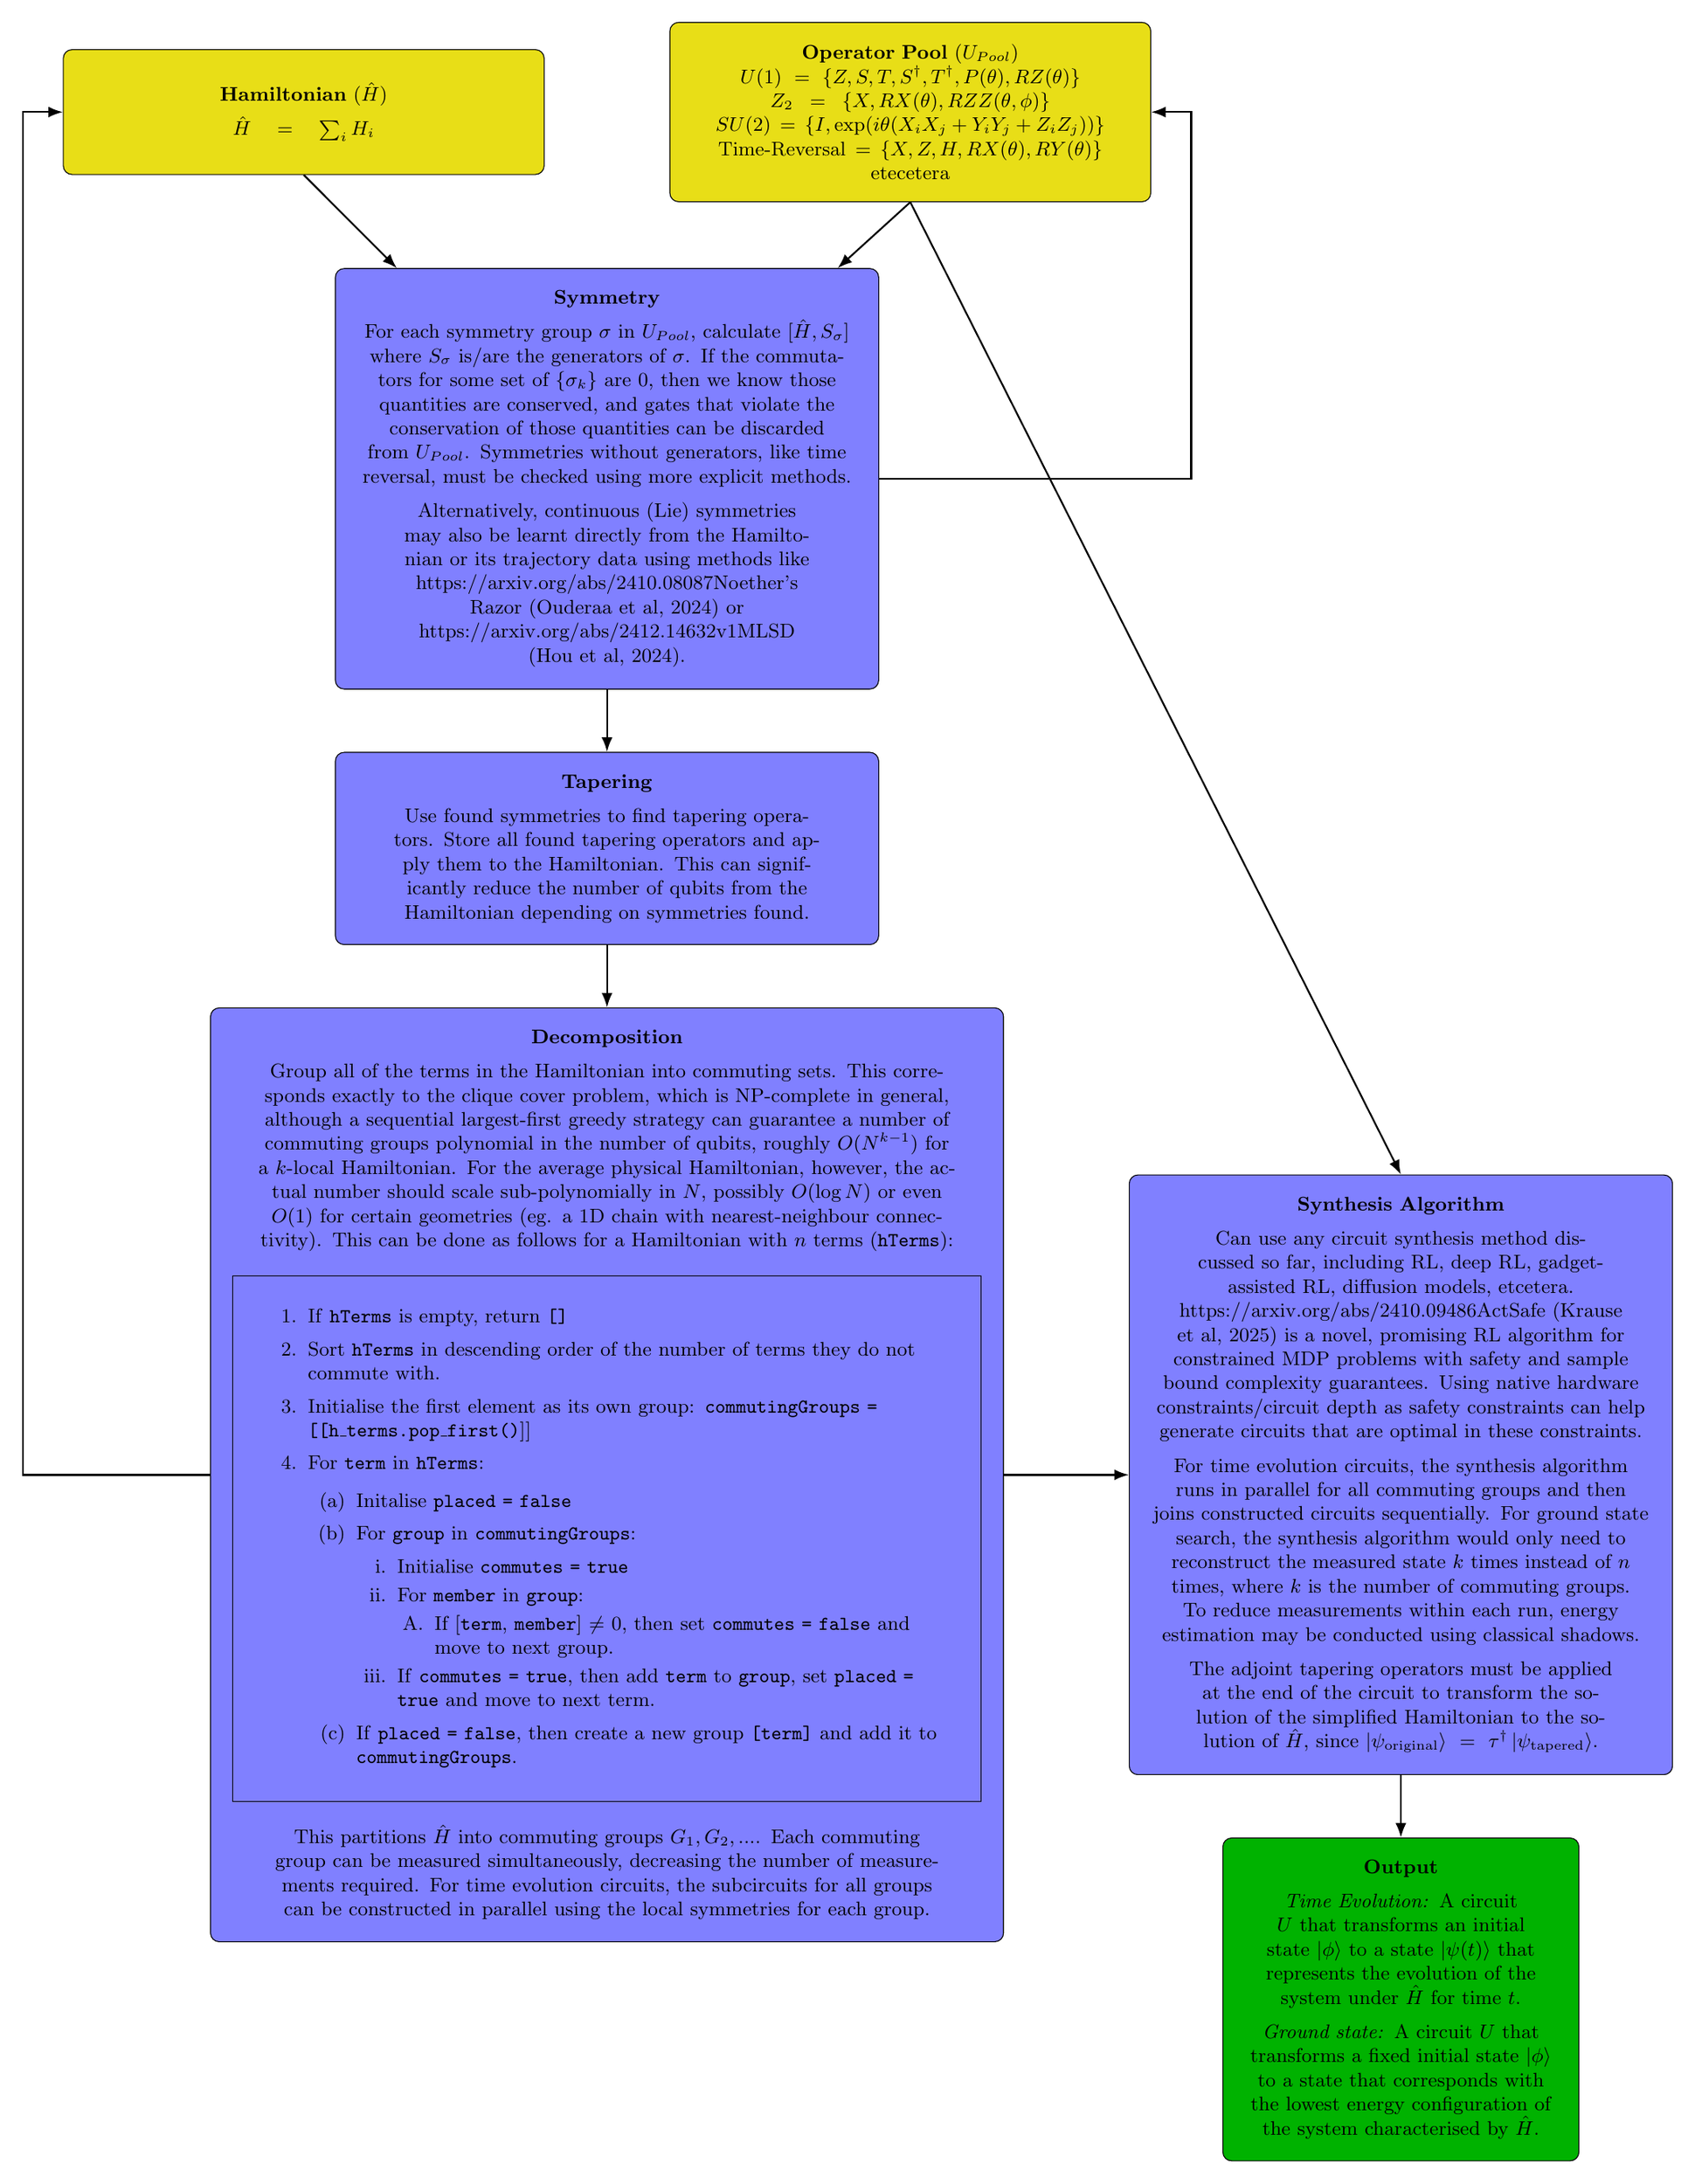
\begin{tikzpicture}[
    input_node/.style={
        draw,
        fill=yellow!90!black, % Dark-ish yellow
        rounded corners,
        text width=7cm,
        align=center,
        inner sep=10pt,
        font=\small,
        minimum height=2cm
    },
    processing_node/.style={
        draw,
        fill=blue!50, % Blue color
        rounded corners,
        text width=8cm,
        align=center,
        inner sep=10pt,
        font=\small,
        minimum height=2cm
    },
    processing_node_decomposition/.style={
        draw,
        fill=blue!50, % Blue color
        rounded corners,
        text width=12cm,
        align=center,
        inner sep=10pt,
        font=\small,
        minimum height=2cm
    },
    label_node/.style={
        font=\bfseries\large,
        align=center
    },
    arrow/.style={
        -Latex,
        thick
    },
    output_node/.style={
        draw,
        fill=green!70!black,
        rounded corners,
        text width=5cm,
        align=center,
        inner sep=10pt,
        font=\small,
        minimum height=2cm
    },
]

% Hamiltonian Node
\node[input_node] (hamiltonian) {
    \textbf{Hamiltonian} ($\hat{H}$) \\
    \vspace{0.5em}
    $\hat{H} = \sum_iH_i$\\
    \vspace{0.5em}
};

% Operator Pool Node
\node[input_node, right=2cm of hamiltonian] (operator_pool) {
    \textbf{Operator Pool} ($U_{Pool}$) \\
    $U(1) = \{Z, S, T, S^\dagger, T^\dagger, P(\theta), RZ(\theta)\}$\\
    $Z_2 = \{X, RX(\theta), RZZ(\theta, \phi)\}$\\
    $SU(2) = \{I, \exp(i \theta(X_i X_j + Y_iY_j + Z_iZ_j))\}$\\
    $\text{Time-Reversal} = \{X, Z, H, RX(\theta), RY(\theta)\}$\\
    etecetera
};

% Symmetry Check Node
\node[processing_node, below=2.5cm of $(hamiltonian)!0.5!(operator_pool)$] (symmetry_check) {
    \textbf{Symmetry} \\
    \vspace{0.5em}
    For each symmetry group $\sigma$ in $U_{Pool}$, calculate $[\hat{H},S_\sigma]$ where $S_\sigma$ is/are the generators of $\sigma$. If the commutators for some set of $\{\sigma_k\}$ are 0, then we know those quantities are conserved, and gates that violate the conservation of those quantities can be discarded from $U_{Pool}$. Symmetries without generators, like time reversal, must be checked using more explicit methods.\\
    \vspace{0.5em}
    Alternatively, continuous (Lie) symmetries may also be learnt directly from the Hamiltonian or its trajectory data using methods like \href{https://arxiv.org/abs/2410.08087}{Noether's Razor} (Ouderaa et al, 2024) or \href{https://arxiv.org/abs/2412.14632v1}{MLSD} (Hou et al, 2024).
};

% Tapering node
\node[processing_node, below= 1cm of symmetry_check](tapering) {
    \textbf{Tapering} \\
    \vspace{0.5em}
    Use found symmetries to find tapering operators. Store all found tapering operators and apply them to the Hamiltonian. This can significantly reduce the number of qubits from the Hamiltonian depending on symmetries found.
};

% Decomposition
\node[processing_node_decomposition, below=1cm of tapering] (decomposition) {
    \textbf{Decomposition} \\
    \vspace{0.5em}
    Group all of the terms in the Hamiltonian into commuting sets. This corresponds exactly to the clique cover problem, which is NP-complete in general, although a sequential largest-first greedy strategy can guarantee a number of commuting groups polynomial in the number of qubits, roughly $O(N^{k-1})$ for a $k$-local Hamiltonian. For the average physical Hamiltonian, however, the actual number should scale sub-polynomially in $N$, possibly $O(\log N)$ or even $O(1)$ for certain geometries (eg. a 1D chain with nearest-neighbour connectivity).
    This can be done as follows for a Hamiltonian with $n$ terms (\hterms):
    \begin{framed}        
    \begin{enumerate}
        \item If \hterms~is empty, return \code{[]}
        \item Sort \hterms~in descending order of the number of terms they do not commute with.
        \item Initialise the first element as its own group: \code{commutingGroups = [[h\_terms.pop\_first()}]]
        \item For \code{term} in \hterms:
        \begin{enumerate}
            \item Initalise \code{placed = false}
            \item For \code{group} in \code{commutingGroups}:
            \begin{enumerate}
                \item Initialise \code{commutes = true}
                \item For \code{member} in \code{group}:
                \begin{enumerate}
                    \item If [\code{term}, \code{member}] $\ne$ 0, then set \code{commutes = false} and move to next group.
                \end{enumerate}
                \item If \code{commutes = true}, then add \code{term} to \code{group}, set \code{placed = true} and move to next term.
            \end{enumerate}
            \item If \code{placed = false}, then create a new group \code{[term]} and add it to \code{commutingGroups}.
        \end{enumerate}
    \end{enumerate}
    \end{framed}
    This partitions $\hat{H}$ into commuting groups $G_1, G_2, ...$. Each commuting group can be measured simultaneously, decreasing the number of measurements required. For time evolution circuits, the subcircuits for all groups can be constructed in parallel using the local symmetries for each group.
};

\node[processing_node, right=2cm of decomposition] (synthesis) {
    \textbf{Synthesis Algorithm} \\
    \vspace{0.5em}
    Can use any circuit synthesis method discussed so far, including RL, deep RL, gadget-assisted RL, diffusion models, etcetera. \href{https://arxiv.org/abs/2410.09486}{ActSafe} (Krause et al, 2025) is a novel, promising RL algorithm for constrained MDP problems with safety and sample bound complexity guarantees. Using native hardware constraints/circuit depth as safety constraints can help generate circuits that are optimal in these constraints.
    \\
    \vspace{0.5em}
    For time evolution circuits, the synthesis algorithm runs in parallel for all commuting groups and then joins constructed circuits sequentially. For ground state search, the synthesis algorithm would only need to reconstruct the measured state $k$ times instead of $n$ times, where $k$ is the number of commuting groups. To reduce measurements within each run, energy estimation may be conducted using classical shadows.\\
    \vspace{0.5em}
    The adjoint tapering operators must be applied at the end of the circuit to transform the solution of the simplified Hamiltonian to the solution of $\hat{H}$, since $\ket{\psi_{\text{original}}} = \tau^\dagger\ket{\psi_{\text{tapered}}}$.
};

\node[output_node, below = 1cm of synthesis](output) {
    \textbf{Output} \\
    \vspace{0.5em}
    \textit{Time Evolution:} A circuit $U$ that transforms an initial state $\ket{\phi}$ to a state $\ket{\psi(t)}$ that represents the evolution of the system under $\hat{H}$ for time $t$.\\
    \vspace{0.5em}
    \textit{Ground state:} A circuit $U$ that transforms a fixed initial state $\ket{\phi}$ to a state that corresponds with the lowest energy configuration of the system characterised by $\hat{H}$.
};

% Arrows
\draw[arrow] (hamiltonian.south) -- (symmetry_check);
\draw[arrow] (operator_pool.south) -- (symmetry_check);
\draw[arrow] (symmetry_check.east) -- ++(5,0) |- (operator_pool.east);
\draw[arrow] (symmetry_check.south) -- (tapering.north);
\draw[arrow] (tapering.south) -- (decomposition.north);
\draw[arrow] (decomposition.west) -- ++(-3, 0) |- (hamiltonian.west);
\draw[arrow] (decomposition.east) -- (synthesis.west);
\draw[arrow] (operator_pool.south) -- (synthesis.north);
\draw[arrow] (synthesis.south) -- (output.north);

\end{tikzpicture}%
    }
    \caption{Workflow Summary}
    \label{fig:summary}
\end{figure}

This paper is structured as follows: Section \RN{2} introduces physical symmetries, their mathematical formalisms, and the methods used to find these symmetries in physical Hamiltonians. It also introduces tapering and twirling, two important operations for reducing the Hilbert space and action space. Section \RN{3} introduces a novel classical algorithm for commutativity-based Hamiltonian partitioning and analyses its runtime complexity and average number of groups with comparisons to existing methods. Section \RN{4} introduces classical shadows, a method introduced in 2020 \cite{huangPredictingManyProperties2020} for measurement-efficient observable expectation value estimation, which is a central technique to ensure measurement efficiency in our approach. Section \RN{5} introduces the circuit synthesis method and its loss function. Section \RN{6} explains the experimental setup used to test the complete framework on $H_2$ and $LiH$ Hamiltonians mapped to qubits using the Jordan-Wigner Transform. Section \RN{7} analyses and discusses the results of the experiments conducted in Section \RN{6}.
Section \RN{8} presents concluding remarks and directions for further research.
	
\section{Symmetries}
	
\subsection{Definitions}\label{ssec:def}
	
\subsubsection{Commutator}
\begin{definition}{Commutator}{comm_def}
	The commutator of two operators $A, B$ is defined as follows:
			
	\begin{equation}
		[A, B] = AB - BA
	\end{equation}
			
	When $[A, B] = 0$, or equivalently, $AB = BA$, the operators $A, B$ are said to commute. \cite{cantwell2016introduction}
	\cite{vonNeumann:2018:MFQ}
\end{definition}
\begin{itemize}
	\item Given some set of observables $\mathcal{A}, \mathcal{B},...$ and their corresponding operators $A, B, ...$, the commutativity of $A, B, ...$ is \textbf{necessary and sufficient} for the simultaneous measurement of $\mathcal{A}, \mathcal{B},...$ \cite{vonNeumann:2018:MFQ}.
	      		
	\item Given a state consisting of $n$ qubits $\ket{\psi} = \bigotimes_{i = 1}^n\ket{\psi_i}$, two spin operators (such as Pauli operators) $I \otimes ...\otimes \sigma^a_j \otimes ... \otimes I$, $I \otimes ...\otimes \sigma^b_k \otimes ... \otimes I$ acting on distinct qubits $a, b$ commute, since the operators act on different factors of the tensor product $\ket{\psi}$ \cite{corry2017symmetry}.
\end{itemize}
\begin{definition}{Anticommutator}{anticomm_def}
	The anticommutator of two operators $A, B$ is defined as follows:
			
	\begin{equation}
		\{A, B\} = AB + BA
	\end{equation}
			
	When $\{A, B\} = 0$, or equivalently, $AB = -BA$, the operators $A, B$ are said to anticommute.
\end{definition}
\subsubsection{Symmetry}
	
Let $X$ be a mathematical object. A symmetry transformation is a mapping $g: X \mapsto X$ that preserves a relevant property of $X$, ie. that property is invariant to $g$. The set of all transformations that preserve this property forms a \textit{group} \cite{cantwell2016introduction}. According to Wigner's theorem, transformations on Hamiltonians that preserve transition probabilities must be unitary or anti-unitary operators \cite{corry2017symmetry}.
	
An operator $U$ is a symmetry of Hamiltonian $\ham$ if it leaves the Hamiltonian invariant, ie. $U\ham U^\dagger =\ham$, which is equivalent to the commutation relation \cite{corry2017symmetry}: \begin{equation}\label{eq:symcom}[\ham, U] = 0\end{equation}
	
\textbf{Discrete Symmetries} are described by discrete groups with finite or countably infinite elements. Some examples of these in quantum mechanics include parity (invariance under spatial inversion), time reversal (invariance under time reversal), etcetera.
	
\textbf{Continuous Symmetries} are described by a Lie group. Any element $U$ of a one-parameter Lie group can be written in terms of a generator $G$ for a continuous parameter $\alpha$: \begin{equation}
U(\alpha) = \exp\left(\frac{i}{\hslash}\alpha G\right)
\end{equation}.
	
If $[\ham, G] = 0$, then the physical quantity represented by $G$ is a \textit{conserved quantity} \ref{def:cq_def}. This is a quantum mechanical statement of Noether's theorem \cite{ouderaaNoethersRazorLearning2024}. An example of this in quantum mechanics is $SU(2)$, which relates to the conservation of total spin.\\
	
\begin{definition}{Conserved Quantity}{cq_def}
	If $O$ is a time-independent observable, then $\ham(t)$ for all times $t$, then for any initial state $\psi$, the expectation value $\braket{O}_{\psi_t}$ is a \textit{conserved quantity} for the dynamics specified by $\ham(t)$.
			
	If $\psi$ is an eigenstate for $O$ such that $O\ket{\psi} = \lambda \ket{\psi}$, then $\psi_t$ is an eigenstate for $O$ with the same eigenvalue $\lambda$ \cite{corry2017symmetry}.
\end{definition}
	
\textbf{Consequences}
\begin{itemize}
	\item If a symmetry operator $U$ does not explictly depend on time, and $[\ham, U] = 0$, then the expectation value of any observable $A$ associated with $U$ is conserved.
	\item If $\ket{\psi}$ is an eigenstate of $\ham$ with eigenvalue $\lambda$, then the state $U\ket{\psi}$ ($U$ is a symmetry operator) is also an eigenstate of $\ham$ with the same eigenvalue $\lambda$.
\end{itemize}

\subsection{Symmetric Operators}
	
\textbf{Symmetry Preservation in Operators}
If an operator $U$ commutes with a symmetry operator $S$ (ie. $[S, U] = 0$) for a Hamiltonian $\ham$, then $U$ preserves the $[\ham, S]$ commutation relation when applied to a state $\ket{\psi}$ evolving under $\ham$, ie. it preserves the symmetry. More precisely, if a state $\ket{\psi}$ is an eigenstate of the symmetry operator $S$ with the eigenvalue $s$, then the new state $\ket{\psi'} = U\ket{\psi}$ is also an eigenstate of $S$ with the same eigenvalue. This is true because: $$S\ket{\psi'} = S(U\ket{\psi}) = U(S\ket{\psi}) = U(s(\ket{\psi})) = s(U\ket{\psi}) = s\ket{\psi'}$$
\vspace{0.1ex}
	
\begin{definition}{Twirling Operator}{tw_def}\label{def:twirl}
	Let $U_s$ be a unitary representation of a symmetry group $\sym$. \begin{equation}\twirl{U}{X} = \begin{cases}\begin{aligned}
	\frac{1}{|S|}\sum_{s \in \sym}U_sXU_s^\dagger & ~~~~\sym \text{ is a discrete group}\\
	\int U_sXU_s^\dagger \dd{\mu} & ~~~~ \sym \text{ is a Lie (continuous) group with Haar measure $\mu$}
	\end{aligned}
	\end{cases}\end{equation}
	defines a projector onto the set of operators commuting with all elements of the representation.\cite{meyerExploitingSymmetryVariational2023}
	To prove this, it suffices to show that $[\twirl{U}{X}, U_s] = 0 ~\forall~ X, s \in \sym$, or equivalently, $U_s \twirl{U}{X}U_s^\dagger = \twirl{U}{X}$. 
	\begin{equation*}
		\begin{split}
			U_s\twirl{U}{X}U_S^\dagger &= U_s\left(\frac{1}{|S|}\sum_{t \in \sym}U_tXU_t^\dagger\right)U_s^\dagger\\
			&= \frac{1}{|S|}\sum_{t \in \sym}U_{st}XU_{st}^\dagger ~~\text{[By the group property $U_sU_t = U_{st}$]}\\
			&= \frac{1}{|S|}\sum_{r \in \sym}U_{r}XU_{r}^\dagger ~~\text{[Relabel $st$ as $r$ (bijective relabeling)]}\\
			&= \twirl{U}{X} ~~~\qed
		\end{split}
	\end{equation*}
			
\end{definition}
	
\textbf{Symmetrising Generators} If an operator $X$ is generated by a generator $G$ from a generator set $\genset$ such that $X = \exp(-i\theta G)$, 
and $\sym$ is a symmetry with unitary representation $U_s$, then $X'$ generated by $G' = \twirl{U}{G}$ commutes with $U$, ie. \begin{equation}
[\exp\left(-i \theta \twirl{U}{G}\right), U_s]= 0 ~ \forall ~ G \in \genset, s \in \sym
\end{equation}
	
Therefore, given a set of generators $\genset$, a gateset constructed as $\mathcal{X} = \{\exp\left(-i\theta\twirl{U}{G}\right)\ | ~G \in \genset \}$ 
is equivariant over symmetry $\sym$ represented by a unitary $U_s, ~s \in \sym$. A circuit constructed from gates in $\mathcal{X}$ is called an \textit{equivariant circuit} for $\sym$.\cite{meyerExploitingSymmetryVariational2023}
	
\subsection{$\zsym$ Tapering}
\subsubsection{$\zsym$ Symmetries}\label{ssec:zsym}
The $\zsym$ group is a cyclic symmetry group of order 2, with elements $\{e, \sigma\}$ where $\sigma\circ\sigma = e$ \cite{Moore2014}. In the context of quantum computing, a $\zsym$ symmetry refers to a unitary operator $\tau$ that commutes with a Hamiltonian $\ham$ and squares to the identity operator, ie. $[\tau_, \ham] = 0$ and $\tau^2 =I$.

For a molecular Hamiltonian mapped to the qubit space using a transform, such as the Jordan-Wigner Transform, the qubit representation is expressed as \begin{equation}\label{eq:hamdef}
    \ham=\sum_jc_j p_j
\end{equation}
Where $c \in \mathbb{C}$, and each $p$ belongs to the Pauli group $P_m = \pm\{I, \sigma^x, \sigma^y, \sigma^z\}^{\otimes n}$ for $n$ qubits. A $\zsym$ symmetry divides the $2^n$-dimensional Hilbert space into two $2^{n-1}$-dimensional sectors corresponding to eigenvalues $+1$ and $-1$ of the symmetry. The correct symmetry sector is then identified using a reference state (typically the Hartree-Fock state).

\textbf{Identifying $\zsym$ Symmetries}
Each Pauli string $p$ acting on $n$ qubits can be parametrised by a binary vector $(a_x|a_z)$ of length $2n$ where each component is either zero or one. The following is an example for a one-qubit system:
\begin{align*}
    I&: (0|0)\\
    X&: (1 | 0)\\
    Y&: (1| 1)\\
    Z&: (0|1)
\end{align*}\\
As another example, take the Pauli string $X \otimes Y \otimes Z$. It can be represented as $(1, 1, 0~|~ 0, 1, 1)$. The Pauli string can thus be obtained as $p(a_x|a_z) = \prod_{i\in a_x}\sigma^i_x \cdot \prod_{j\in a_z}\sigma^j_z$. Two Pauli strings commute if $a_zb_x + a_xb_z \mod 2= 0$\cite{setiaReducingQubitRequirements2020}. 

The Pauli strings in a Hamiltonian can be represented as $G(\ham) = \left[\frac{G_x}{G_z}\right]$ where the $\th{j}$ column corresponds to $(a_x | a_z)$ representing $p_j$. From this matrix, we can construct the check matrix $E = [(G_z)^T | (G_x)^T]$. The kernel $\ker(E)$ thus gives us the generators $\tau_i$ of the group using Gram-Schmidt orthogonalisation over the binary field $GF(2)$.

\begin{framed}\label{z2example}
\textbf{Example 1}
\begin{align*}
    \ham &= X\otimes Y + Y \otimes Z + X \otimes X\\
    &= (1, 1 | 0, 1) + (1, 0 | 1, 1) + (1, 1 | 0, 0)\\
    G(\ham) &= \begin{bmatrix}
    1 & 1 & 1\\
    1 & 0 & 1\\
    0 & 1 & 0\\
    1 & 1 & 0
    \end{bmatrix}\\
    E &= \begin{bmatrix} 
    0 & 1 & 1 & 1\\
    1 & 1 & 1 & 0\\
    0 & 0 & 1 & 1
    \end{bmatrix}\\
    \ker(E) &= \{[1, 0, 1, 1]\}\\
    [1, 0, 1, 1] &\mapsto Y \otimes Z\\
    \therefore \tau = Y \otimes Z &\text{ is a generator of $\zsym$ symmetry for $\ham$}.\\\\
    \text{This can be } & \text{verified by finding $[\tau, \ham]$}:\\
    [\tau, \ham] &= \tau \ham - \ham \tau\\
    &= Y \otimes Z (X\otimes Y + Y \otimes Z + X \otimes X) \\&~- (X\otimes Y + Y \otimes Z + X \otimes X) Y \otimes Z\\
    &= -Z \otimes X + I \otimes I + Z \otimes Y \\&~+ Z \otimes X - I \otimes I - Z \otimes Y\\
    &=0
\end{align*}
\end{framed}

\subsubsection{Tapering}

Consider a set of $k$ qubits on which all the terms of a Hamiltonian $\ham$ ($\{p_j\}$) act trivially (ie. $I$). Then, it is easy to see that we can remove those $k$ qubits from our simulation. This is also true if the Hamiltonian acts with at most one Pauli gate (eg. $\sigma_x$) on the $k$ qubits. In this scenario, the single-qubit Pauli gate appearing in the $p_j$ terms can be replaced by their eigenvalues $\pm 1$, so that the $\th{j}$ qubit can be tapered off \cite{setiaReducingQubitRequirements2020}.

From stabiliser theory, we know that every group has a set of generators $\{\tau_1, ..., \tau_k\}$, and that there exists a unitary $U_i$ for each $\tau_i$ such that\cite{setiaReducingQubitRequirements2020}:
\begin{equation}\label{eq:stabtheory}
    U_i\tau_iU_i^\dagger = \sigma_x^{q(i)}
\end{equation}

Where $q(i)$ refers to the index of the qubit on which the $\tau_i$ is mapped to a single-qubit $\sigma_x$ operator after conjugation by $U_i$, and $U_i$ belongs to the Clifford group, which maps the set of $n$-fold Pauli operators onto itself. Notice that $U_i$ is Hermitian and unitary, ie. $U_i= U_i^{\dagger}$. Therefore, if we find the set of $\zsym$ symmetries of a Hamiltonian $\ham$, then we can transform the set of symmetry generators to single-qubit $\sigma_x$ operators using \eqref{eq:stabtheory}.\\
For each symmetry $\tau_i$ for Hamiltonian $\ham$, if we transform the Hamiltonian using the corresponding unitary $U_i$, then each Pauli term in the transformed Hamiltonian must commute with $\sigma_x^{q(i)}$. This can be shown as follows:\\
\begin{align*}
    \ham ' &\coloneq  U_i \ham U_i^\dagger &[\text{Definition 1}]\\
    &= \sum_j c_j U_i p_j U_i^\dagger &[\text{From \eqref{eq:hamdef}}]\\
    &= \sum_j c_j p'_j ~~\{p'_j \in P_m\}&[\text{From def. of Clifford group}]\\
    [\tau, \ham]&=0 &[\text{From \eqref{eq:symcom}}]\\
    [U_i\tau U_i^\dagger, U_i\ham U_i^\dagger]&=0  &[\text{Conjugation by $U_i$}]\\
    [\sigma_x^{q(i)}, \ham'] &= 0 &[\text{From \eqref{eq:stabtheory}, Definition 1}]\\
    \therefore [\sigma_x^{q(i)}, p'_j] &= 0 ~\forall ~j&\text{[By Definition 1]}&~~\qed
\end{align*}

This implies that the transformed Hamiltonian is acting trivially or at most with $\sigma_x$ on the $\th{q(i)}$ qubit. This allows us to replace the $\sigma_x^{q(i)}$ by its eigenvalue, and thus remove the qubit from the system \cite{setiaReducingQubitRequirements2020}.

Once we have the $\zsym$ symmetries $\{\tau_1, .. \tau_k\}$ obtained as described in section \ref{ssec:zsym}, each of these symmetries can be converted into a $\sigma_x$ operator acting on a single qubit using their corresponding $U_i$. To find this unitary for each symmetry $\tau_i$, we find the $\sigma_x$ on a qubit such that it anticommutes with $\tau_i$ and commutes with the other symmetries. Then, $U_i$ is given by\cite{setiaReducingQubitRequirements2020} \begin{equation}\label{eq:taperunit}
    U_i =\frac{1}{\sqrt2}\left(\tau_i + \sigma_x^{q(i)}\right)
\end{equation}

We can verify this using the Hamiltonian and symmetry from our previous example 1 \ref{z2example}.
\begin{framed}\label{taperexample}
\textbf{Example 2}
\begin{align*}
    \ham &= X\otimes Y + Y \otimes Z + X \otimes X\\
    \tau &=Y \otimes Z\\
    \sigma_x^{trial} &\coloneq I \otimes X\\
    \{I \otimes X, Y \otimes Z\} &= (I \otimes X)(Y \otimes Z) + (Y \otimes Z)(I \otimes X)\\
    &=0\\
    \therefore q(1) &= 2\\
    \implies U_1 &= \frac{1}{\sqrt2} \left(Y\otimes Z + I \otimes X\right)\\\\
    \text{Applying this } & \text{unitary to our symmetry generator,}\\
    U_1 \tau_1 U_1^{\dagger} &= \left(\frac{1}{\sqrt2} \left(Y\otimes Z + I \otimes X\right)\right)(Y\otimes Z) \left(\frac{1}{\sqrt2} \left(Y\otimes Z + I \otimes X\right)\right)\\
    &= \frac{1}{\sqrt2}\left(I \otimes I - i Y \otimes Y\right)\left(\frac{1}{\sqrt2} \left(Y\otimes Z + I \otimes X\right)\right)\\
    &= \frac{1}{2}\left(Y \otimes Z + I \otimes X + I \times X - Y\otimes Z\right)\\
    &= I \otimes X\\
    \implies \text{The } &\text{unitary correctly transforms $\tau_1$ to a single-qubit $\sigma_x$}\\\\
    \text{Applying this } & \text{unitary to our Hamiltonian,}\\
    \ham' &= \left(\frac{1}{\sqrt2} \left(Y\otimes Z + I \otimes X\right)\right)(X\otimes Y + Y \otimes Z + X \otimes X)\left(\frac{1}{\sqrt2} \left(Y\otimes Z + I \otimes X\right)\right)\\
    &= \frac{1}{2}\left(2 X\otimes X - 2 Z \otimes I + 2 I \otimes X\right)\\
    &= X \otimes X + I \otimes X - Z\otimes I\\
    \text{This gives us a $\ham'$}&\text{ with at most one $\sigma_x$ operation on the second qubit,}\\
    \text{so it can be } & \text{tapered off by replacing $\sigma_x$ operations with $\pm1$.}\\
    \therefore \ham'_{\pm 1}&=\begin{cases}X+I-Z & \text{Eigenvalue = $+1$}\\-(X+Z+I)&\text{Eigenvalue = $-1$}\end{cases}
\end{align*}
\end{framed}
{\footnotesize Note that we could have chosen either qubit to taper off for this case. This is not true in general. All the qubits may have to be tested for this tapering process.}\\\\
Thus, we have reduced a Hamiltonian acting on two qubits to one acting on a single qubit. The symmetry sector can be chosen based on a reference state, such as the Hartree-Fock State \cite{setiaReducingQubitRequirements2020}.


\subsection{Common Physical Symmetries}

\subsubsection{$U(1)$ Symmetry}

The $U(1)$ symmetry is a Lie group that geometrically corresponds to the circle group. Under the Jordan-Wigner Transform, the $U(1)$ symmetry corresponds to the conservation of particle number, which is tantamount to the conservation of the number of qubits in the excited state $\ket{1}$ \cite{gardEfficientSymmetrypreservingState2020}. For example, a system with $n$ electrons and $m$ orbitals is invariant to the $U(1)$ symmetry if and only if $n$ is conserved \cite{Mbeng2024Quantum_Ising}.

It can be shown that the generator corresponding to this symmetry is $U_{U(1)} =\sum_{j=1}^MZ_j$.
\begin{align*}
    \text{From \cite{Mbeng2024Quantum_Ising}, we have } Z_j &= 1-2\hat{n}_j \text{ where $\hat{n}_j$ is the particle number operator for orbital $j$.}\\
    \implies \hat{n}_j &= \frac{1 - Z_j}{2}\\
    \implies \hat{N} &= \sum_{j = 1}^M \frac{1 - Z_j}{2} \text{ where $\hat{N}$ is the total particle number operator over all orbitals}\\
    &=\frac{1}{2}\left(\sum_{j=1}^{M} 1 - \sum_{j=1}^M Z_j \right)\\
    &=\frac{1}{2}\left(M - \sum_{j=1}^M Z_j \right)\\
    \text{The condition for } &\text{conservation of total particle number is $\left[\ham, \hat{N}\right] = 0$}
\end{align*}\vspace{-1.5em}
\begin{align*}
    &\implies \left[\ham, \frac{1}{2}\left(M - \sum_{j=1}^M Z_j \right)\right] = 0\\
    &\implies \frac{1}{2}\left[\ham, M - \sum_{j=1}^M Z_j \right] = 0 & \text{[Factor out constant]}\\
    &\implies \frac{1}{2}\left(\left[\ham, M\right] - \left[ \ham, \sum_{j=1}^M Z_j \right]\right) = 0 & \text{[By distributive property of commutation]}\\
    &\implies -\frac{1}{2}\left[ \ham, \sum_{j=1}^M Z_j \right] = 0 & \text{[$M$ is scalar, which commutes with $\ham$]}\\
    &~~~~U_{U(1)} \coloneq\sum_{j=1}^M Z_j&\\
    &\therefore \left[ \ham, U_{U(1)} \right] = 0~~\qed \\
\end{align*}

Therefore, a generator $G$ can be symmetrised by twirling it with respect to the operators in the symmetry group, $U_{U(i)}$ \ref{eq:taperunit}.
\begin{equation}
    \twirl{U_{U(1)}}{G} = \frac{1}{2\pi}\int_0^{2\pi} V(\theta)GV^\dagger(\theta) d\theta
\end{equation}

Where $V(\theta) = \exp(-i\theta U_{U(i)}), V^\dagger(\theta) = \exp(i\theta U_{U(i)})$

\subsubsection{$SU(2)$ Symmetry}

$SU(2)$ symmetry is a Lie group that geometrically corresponds to the 3-sphere. Under the Jordan-Wigner Transform, the $SU(2)$ symmetry corresponds to the conservation of total spin.  

Define the components of the total spin as:
\begin{equation}
S_\alpha = \frac{1}{2}\sum_i\alpha_i~~~~~\alpha \in \{\sigma_x, \sigma_y, \sigma_z\}\    
\end{equation}

If a Hamiltonian $\ham$ commutes with $S_x$, $S_y$, and $S_z$, ie.

\begin{equation}\label{eq:su2symcon}
    [\ham, S_x] = [\ham, S_y] = [\ham, S_z] = 0
\end{equation}

Then it can be shown that $\ham$ is invariant to any arbitrary rotation in spin space:

Let an arbitrary rotation be represented by a unitary $\urot(\hat{n}, \theta) = \exp(-i \theta \hat{n}\cdot \vec{S}/\hslash)$ where:
\begin{itemize}
    \item $\theta$ is the angle of rotation
    \item $\hat{n} = (n_x, n_y, n_z)$ is a unit vector defining the axis of rotation.
    \item $\vec{S} = (S_x,S_y,S_z)$ is the vector of total spin operators.
    \item Set $\hslash= 1$ without loss of generality.
\end{itemize}

Given eq. \eqref{eq:su2symcon}, we must show that $[\ham, \urot] = 0$ for any arbitrary $\urot$. To do this, we first show that $\ham$ commutes with the spin operator along an arbitrary direction. Then, we show that $\ham$ commutes with $\urot$ using its Taylor series representation.

\begin{align*}
S_n&\coloneq \hat{n} \cdot \vec{S} = n_xS_x + n_yS_y+n_zS_z & \text{[$S_n$ is the projection of the spin vector along $\hat n$]}\\
[\ham, S_n] &= [\ham , n_xS_x + n_yS_y+n_zS_z]\\
&= n_x[\ham, S_x] + n_y[\ham, S_y] + n_z[\ham, S_z] &\text{[Using linearity, since $n_x, n_y,n_z$ are scalars]}\\
&= n_x \times 0 +  n_y \times 0 +  n_z \times 0 = 0 &\text{[By construction \eqref{eq:su2symcon}]}\\
\therefore [\ham, S_n] &=0
\end{align*}
\begin{align*}
    \urot &= \exp(-i\theta S_n) = \sum_{k=0}^\infty\frac{(-i\theta)^k}{k!}(S_n)^k &\text{[Taylor Series of $\urot$]}\\
    [\ham, \urot] &= \left[\ham, \sum_{k=0}^\infty\frac{(-i\theta)^k}{k!}(S_n)^k \right]\\
    &= \sum_{k=0}^\infty\frac{(-i\theta)^k}{k!}\left[\ham,(S_n)^k \right] &\text{[Linearity of commutator]}\\
    &=\sum_{k=0}^\infty\frac{(-i\theta)^k}{k!}\times 0 &\text{[From previous result]}\\
    &= 0\\
    \therefore [\ham, \urot] &= 0 ~~\qed
\end{align*}

A generator $G$ can be symmetrised by twirling it with respect to the operator of the symmetry group, $\urot$. By parametrising $\urot$ with Euler angles $\alpha, \beta, \gamma$, the twirl can be shown to be \cite{shankar1994principles}:

\begin{equation*}
    \twirl{\urot}{G} = \frac{1}{16\pi^2}\int_0^{2\pi}\int_0^{2\pi}\int_0^{2\pi}\urot(\alpha, \beta,\gamma)G\urot^\dagger(\alpha, \beta,\gamma)\sin\beta~ d\alpha~ d\beta ~d\gamma
\end{equation*}

This is evidently not a practical equation to solve. However, it is known that for spin-$1/2$ systems, we can replace this integral by a discrete sum over the Clifford group \cite{tdesign}, ie.

\begin{equation}
    \twirl{\urot}{G} = \twirl{\text{Clifford}}{G} = \frac{1}{|\text{Clifford}|}\sum_{C \in \text{Clifford}}CGC^\dagger
\end{equation}

\subsubsection{Time-Reversal Symmetry}

$TRS$ is a discrete symmetry wherein the fundamental laws governing the system do not distinguish between the forward and backward flow of time \cite{Sakurai_modern_qm2010}. 

For spin-$1/2$ systems, the $TRS$ operator is the antiunitary \cite{Sakurai_modern_qm2010}:
\begin{equation}
    T = (-i\sigma_y)K
\end{equation}

Where $K$ denotes complex conjugation in the computational basis. Operator $T$ transforms the Pauli operators as follows:
\begin{equation}\label{eq:sigmatransform}
    T\sigma_\alpha T^\dagger = -\sigma_\alpha ~~\alpha \in \{x, y,z\}
\end{equation}

A Hamiltonian $\ham = \sum_{r=1}^m c_rp_r$ is time-reversal symmetric if and only if $T\ham T^\dagger = \ham$. However, if $c_r \in \mathbb{R} ~\forall~ r \in [1, m]$, then we can show that $T\ham T^\dagger = \ham \iff W(p_r) \mod 2=0 ~~\forall~~r \in [1, m]$ where $W(p)$ is the weight of the Pauli string, ie. the number of non-identity Pauli operators present in the string.

\begin{align*}
    T\ham T^\dagger &= \sum_{r=1}^m Tc_rT^\dagger \cdot Tp_rT^\dagger\\
    &= \sum_{r=1}^mc_r Tp_rT^\dagger &\text{[$c_r$ terms are real scalars]}\\
    \text{Thus, it } & \text{suffices to show that } T p_r T^\dagger = p_r ~~\forall~~ r \in [0, m]\\
    Tp_rT^\dagger &= T(\sigma_{\alpha}^1 \otimes \dots\otimes \sigma_{\alpha}^{W(p_r)})T^\dagger\\
    &= (T\sigma_{\alpha}^{1}T^\dagger)\otimes\dots\otimes (T\sigma_{\alpha}^{W(p_r)}T^\dagger)\\
    &= (-\sigma_{\alpha}^{1})\otimes\dots\otimes (-\sigma_{\alpha}^{W(p_r)}) &\text{[From Eq. \eqref{eq:sigmatransform}]}\\
    &= (-1)^{W(p_r)}p_r\\
    \iff W(p_r) &= 2k,~~k \in \mathbb{Z^+}\\
    \therefore W(p_r) \mod 2&= 0 ~~\forall~~ r\in [1, m]~~\qed
\end{align*}

We can also deduce in the general case of $c_r \in \mathbb{C}$, then the following conditions suffice for $TRS$:
\begin{enumerate}[(1)]
    \item Even-weight strings have purely real coefficients.
    \item Odd-weight strings have purely imaginary coefficients.
    \item If an even-weight Pauli string has a non-real coefficient, or if an odd-weight Pauli string does not have a purely imaginary coefficient, then $\ham$ must contain both the original term and its time-reversed counterpart (ie. mapped by complex conjugation and possible sign-flip).
\end{enumerate}

Since $T$ is an antiunitary rather than a unitary as required by def. \ref{def:twirl}, we cannot use the Twirling superoperator to symmetrise our generators. We must instead calculate $\genset_{TRS}=\{G \in \genset :  [G, T] = 0$\} to find the generators that commute with $T$.

\subsubsection{Other Symmetries To Be Considered}
\begin{itemize}
    \item SO(3)
    \item Permutation
    \item Parity
\end{itemize}
	
\section{Partitioning}

Let $\ham$ be a $k$-local Hamiltonian (ie. each term acts on at most $k$ qubits) acting on $n$ qubits with $m$ terms. If the Hamiltonian can be partitioned into $q$ groups of commuting Pauli strings, then the observables in each group can be measured simultaneously \ref{ssec:def} for efficient measurement.\begin{equation}
    \ham = \sum_{i=1}^q G_i = \sum_{i=1}^q\sum_r c_rp_r
\end{equation}

This partition problem corresponds exactly to the minimum graph colouring and minimum clique cover problems, making it NP-complete in general. Since we want to minimise the number of commuting groups without brute force, this problem can be approximately solved by a modified Recursive Largest-First algorithm that adds some classical performance cost in exchange for more optimal groups \cite{adegbindin2016}. We represent $\ham$ as a non-commuting graph $\genset = (V,E)$ where $V$ corresponds to the Pauli strings $\{p_1, ..., p_m\}$, and $E = \{(p_i, p_j) : [p_i, p_j] \neq 0\}$.

The selection criterion is the $B(u)$ criterion: For vertex $u$ in the set of available candidates and current independent set $S$, 
\begin{equation}
    B(u, S) = |\{v \in N(u) ~\cap ~\text{unassigned} : v \not \in N(S)\}|
\end{equation}
Where:
\begin{itemize}
    \item $N(u)$ = neighbours of vertex $u$ in the commutator graph.
    \item $\text{unassigned}$ is the set of vertices (Pauli strings) that have not been assigned to a commuting group.
    \item $N(S) = \bigcup_{s \in S}N(s)$, the union of the neighbours of the vertices in $S$.
\end{itemize}

Intuitively, $B(u)$ counts the number of neighbours of $u$ that could potentially be added to the same group as $u$ in future iterations. This can be computed in $O(m)$ if given a method to check commutation in $O(1)$, such as a commutation table \cite{adegbindin2016}.

\begin{longtable}{p{10cm} | p{6cm}}\label{tab:groupingsteps}
\textbf{Steps} & \textbf{Runtime Complexity}\\
\hline\\
\textbf{Commutation Table: }
Build a commutation table where entry $(i,j)$ is $1$ if $[p_i, p_j] = 0$ and $0$ otherwise. & $O(m^2) \text{ [check $m \times m$ pairs] } \times O(k) \text{ [find commutator for pair] } = O(km^2)$\\\\
\textbf{Enhanced RLF}:
\begin{enumerate}
    \item Initialise all Pauli terms as unassigned.
    \item While there are unassigned terms:
    \begin{enumerate}
        \item Start a new group $G$.
        \item Select an unassigned Pauli term with the largest number of non-commuting partners (ie. largest degree from the graph $\genset$) and add it to $G$.
        \item For each remaining unassigned item $u$, check if it commutes with every term in $G$.
        \begin{enumerate}
            \item If yes, compute its $B(u, G)$.
            \item Select the term with the highest $B(u,G)$ to $G$.
        \end{enumerate}
        \item Repeat until no more terms can be added to $G$ without breaking commutativity.
        \item Mark all items in $G$ as assigned.
    \end{enumerate}
\end{enumerate} &$O(m) \text{ [loop over unassigned] } \times O(m) \text{ [loop over other unassigned] } \times O(m) \text{ [$B(u,G)$] } = O(m^3)$\\\\
\textbf{Clique Optimisation}:
\begin{enumerate}
    \item Identify all groups with size below a certain threshold $t$ and collect them into a single pool $S$ of size $s$. Mark them as unassigned.
    \item Create a commuting graph $\genset'$ of $S$ where $V = \{p_s: s \in S\}, E = \{(p_i, p_j):[p_i, p_j]= 0\}$
    \item Use Bron-Kerbosch maximal clique search algorithm to find the maximal cliques \cite{BKAlgo}.
    \item Add each clique found as a new group and mark each item in the clique as assigned.
\end{enumerate} & $O(3^{s/3})$ [Bron-Kerbosch]. In general, $s \in O(m)$. However, $t$ is typically small, so $s << m$.
\end{longtable}

The runtime complexity for the above algorithm is:\begin{equation*}
    O(km^2) + O(m^3) + O(3^{s/3})
\end{equation*}
Since $k \le n, s << m$, the worst-case runtime is
\begin{equation}O(nm^2 + m^3)\end{equation}

The theoretical upper bound on the number of groups is \begin{align}
    \chi(\genset)&\le m\\
    \chi_{\text{RLF}}(\genset)&=\delta(\genset) + 1 \le 4^k \le 4^n
\end{align}
Where $\delta(\genset)$ is the degeneracy of the graph. For the average physical Hamiltonian, however, the actual number should scale sub-polynomially in $n$, possibly $O(\log n)$ or even $O(1)$ for certain geometries (eg. a 1D chain with nearest-neighbour connectivity).

\printbibliography
\end{document}